\documentclass{beamer}
\usepackage{icomma}
\usepackage{tikz}
\usepackage{caption}

\usetikzlibrary{positioning}
\usetikzlibrary{calc}
\usetikzlibrary{shapes, positioning, arrows.meta, fit}
\captionsetup{justification=centering}

\usetheme{Copenhagen}
\usecolortheme{default}
\setbeamertemplate{navigation symbols}{}
\setbeameroption{show notes on second screen=right} % Both
\setbeamertemplate{note page}{\pagecolor{yellow!5}\insertnote}

\DeclareMathOperator*{\argmax}{arg\,max} 
\DeclareMathOperator*{\argmin}{arg\,min}
\newcommand{\indep}{\perp \!\!\! \perp}
\newcommand\norm[1]{\lVert#1\rVert}
\newcommand{\q}{q}
\newcommand{\ml}{k}
\newcommand{\btheta}{\theta}
\newcommand{\la}{\psi}
\newcommand{\Sn}{S^n}
\newcommand{\lib}{\Psi}
\newcommand{\lone}{\mathcal{L}}
\newcommand{\empmod}{\mathcal{P}_{\text{emp}}}
\newcommand{\meta}{\phi}
\newcommand{\Meta}{\Phi}
\newcommand{\esl}{\Sigma}
\DeclareMathOperator{\expit}{expit}




% \title[About Beamer] %optional
\title{Super Learners}
\subtitle{and their oracle properties}
\author[Jinyang Liu (sqf320)]{Jinyang Liu (sqf320)}

\institute[UCPH] % (optional)
{
  Department of Mathematical Sciences\\
  University of Copenhagen
}

\date[VLC 2023]{June 2023}


%End of title page configuration block
%------------------------------------------------------------
%The next block of commands puts the table of contents at the 
%beginning of each section and highlights the current section:

\AtBeginSection[]
{
  \begin{frame}
    \frametitle{Overview}
    \tableofcontents[currentsection]
  \end{frame}
}

\setbeamertemplate{headline}{}
%------------------------------------------------------------
\begin{document}


\frame{\titlepage}
%---------------------------------------------------------
\section{Introduction}

% binary regression maps to probability interval
% differs from binary classification in that the prediction is continuous
% Remark on notation R(\btheta, P)
\begin{frame}
    \frametitle{Binary regression}
    Let $ O = (Y, X) \sim P\in\mathcal P $ be an observation where $ Y \in \{0,1\} $ is our \textbf{outcome} and $ X \in\mathcal X \subseteq \mathbb{R}^{d} $ is our \textbf{covariates}.
    \vfill
    The set of \textbf{regression functions} is
    $$ \Theta = \{\btheta \mid \btheta : \mathcal{X} \to [0,1] \text{ measurable}\}.$$
    \vfill
    The mean squared error (MSE) or \textbf{risk} of \(\btheta \in \Theta\)
        $$
            R(\btheta , P) = \int (Y - \theta(X))^2 d P,
        $$
        is minimized by the conditional expectation referred to as the \textbf{true regression}
    $$ x \mapsto E(Y \mid X = x) = P(Y = 1 \mid X = x). $$ 
    \note{
    We will consider the case of binary regression, where an observation consists of a binary outcome Y and covariates X. The observation is distributed according to P which comes from statistical model 

    Binary regression estimates the probability of Y being equal to 1 given the covariates X. It differs from binary classification in that the prediction is continuous.

    We consider a set of regression functions that map from our covariates to the probability interval, which are the functions we use to predict the probability. 

    A way to evaluate the regression functions is to consider the MSE or risk, which we denote as R theta P, and is the integral of squared difference between Y and theta applied on X wrt. to P. 

    However, we can never calculate the true MSE in the form above directly, since it depends on P, which is unknown.

    It turns out, that the MSE is minimized by the conditional expectation, which we refer to as the true regression. 

    our goal is therefore to estimate the true regression, one way is to assume... 

    problem is that our assumptions are frequently incorrect, and we risk misspecifying the model so it is tempting to use nonparametric machine learning methods which are less biased.

    We now introduce some terminology
    }
\end{frame}
% our goal is therefore to estimate the conditional expectation, to do so
% we assume certain things about the statistical family P, for example that it is a exponential family, and then we can estimate the parameters via maximum likelihood and give an analytic expression of the estimated regression 
% problem is that our assumptions are frequently incorrect, and we risk misspecifying the model so it is tempting to use nonparametric machine learning methods instead which are less biased

\subsection{Terminology}
\begin{frame}
    \frametitle{Terminology}
    Let $ D_n = (O_1 , \dots , O_n) \in \mathcal{O}^{n}$ be the \textbf{data}. %upon which we apply our \textbf{learning algorithms}  
    \begin{block}{Learning algorithm}
        A learning algorithm is a measurable map $ \la : \mathcal{O}^{n} \to \Theta $ for $ n \in \mathbb{N} $. 
      \end{block}
      \vfill
      % We assume that the $ \la $ is well-defined for all $ n \in \mathbb{N} $ and that the ordering of the observations does not matter.
    \begin{block}{Learner or fitted learner}
        A learner $ \la(D_n)\in \Theta$ is the outcome of applying $ \la $ to the data $ D_n $.
      \end{block}
      \vfill
    We usually have a \textbf{library of $ k $ learning algorithms}, 
    \begin{align*}
        \lib = \{\la_{\q} \mid 1 \leq \q \leq\ml \},
    \end{align*}
    which we can use to estimate \(P(Y = 1 \mid X=x)\).
    \note[item]{Let Dn be the data which consists of the observations from 1 up to n}
    \note[item]{A learning algorithm, denoted as psi, is a map from the data to the set of regression functions}
    \note[item]{A learner is then simply the outcome of applying the learning algorithm to the data}

    \note[item]{A learning algorithm could for example be logistic regression, or a neural network}

    \note[item]{In machine learning, the algorithm is fitted or trained on the observed data, and the outcome is a a fitted model, which is used to predict on new covariates}
    \note[item]{we usually have a library of learning algorithms at our disposoal, which we can use to estimate the true regression}
\end{frame}

\begin{frame}
    \frametitle{Two learners: Logistic Regression and XGBoost} 
    \begin{figure}
        \centering
        \centerline{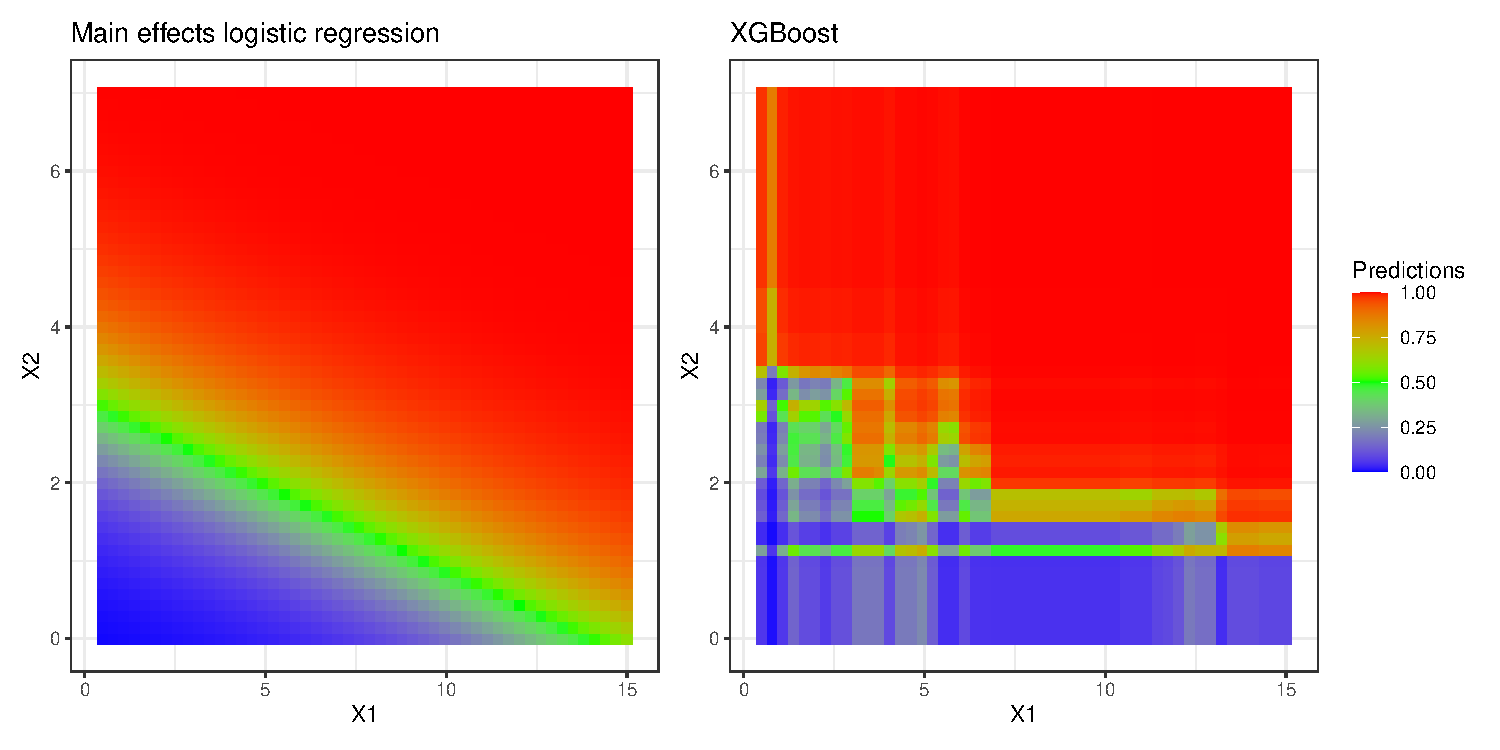
\includegraphics[width=1.1\textwidth]{figures/predictpar.pdf}}
        \caption{The predictions of the main effects logistic regression and XGBoost fitted on $ 1,000 $ observations.}
        \label{fig:predictpar2}
    \end{figure}
    \note[item]{As an example, we can consider logistic regression and the gradient-boosting tree-based algorithm XGBoost.}

    \note[item]{Here we have two covariates X1 and X2 and a binary outcome, the two algorithms are fitted on 1000 observations and are used to predict on the covariates in a grid}

    \note[item]{the predicted probabilities are colored from 0 up to 1}

    \note[item]{We see that there's a huge difference in the pattern of predicted probabilities by the two algorithms}

    \note[item]{Logistic regression, which assumes that the statistical model is binomial has a much smoother pattern than XGBoost, which since it is based on decision trees, predicts the probability in a patchy pattern}

    \note[item]{A natual question arises which is how do we determine the best learning algorithm from looking at the predictions?}

    \note[item]{Given that we do not know the data-generating distribution P, it is not possible to say if any of the algorithms has correctly estimated the regression}

    \note[item]{It might be the case that the true regression is pathological, and assumes the irregular pattern that XGBoost has estimated}

    \note[item]{But this seems improbable in a real-world scenario, and one might believe that it is more smooth as assumed by the logistic regression }

    \note[item]{A way to evaluate the algorithms is to do K-fold cross-validation}
\end{frame}

\subsection{Cross-validation}
\begin{frame}
\frametitle{$ K $-fold Cross-validation}
There is a one-to-one correspondence between our data $ D_n $ and the empirical measures over $ n $ observations
\begin{align*}
    P_n = \sum_{i = 1}^{n} \delta_{O_i},
\end{align*}
$ K $-fold cross-validation splits $ D_n $ into $ K $ \textbf{validation} and \textbf{training} sets. The splits are indexed by $ s \in \{1, \dots , K\} $ and we denote the empirical measures over the validation and training sets of split $ s $ as 
\begin{align*}
    P_{n,s}^{1} := \frac{1}{n_1} \sum_{i: s(i) = s} \delta_{O_i}, \qquad P_{n,s}^{0} := \frac{1}{n_0} \sum_{i: s(i) \neq s} \delta_{O_i}. 
\end{align*}
Here $ s(i) $ denotes the split $ s $ where $ O_i$ is in the validation set of $ s $, and $ n_1, n_0 = n - n_1 $ are the number of observations in the validation and training sets respectively. 

\note[item]{We first note that there is a one-to-one correspondence between the data and the empirical measures over n observations}

\note[item]{Where the delta O i is the dirac measure over O i}

\note[item]{Indeed, from the observations we can construct the empirical measures, and by knowing the empirical measures we also know our observations}

\note[item]{The learning algorithms was a function of the data, but can just as well a function of the empirical measures due to this correspondence}

\note[item]{K-fold cross-validation splits the data in validation and training sets ..}

\note[item]{s of i denotes the split s where observation i is in the validation set s. The variable s really just indexes the validation sets, since for each s you have a validation set that is disjoint from all other validation sets, here the training set is the observations complement of the validation set}
\end{frame}

\begin{frame}
\begin{exampleblock}{The \textbf{super learner} $ K $-fold cross-validation procedure}
  % The \textbf{super learner} uses cross-validation:
  \begin{enumerate}
        \item Randomly split $ D_n $ into $ K $ disjoint and exhaustive validation sets
        \item For each $ s \in \{1, \dots , K\} $ fit each $ \la \in \lib $ on the training data $ P_{n, s}^{0} $ and obtain $ \la(P_{n, s}^{0}) $ 
        \item For each \(s\) and $ \la $, use $ \la(P_{n, s}^{0}) $ to predict on the validation set to obtain \textbf{level-1 covariates}:
          $$ Z_i = \left(\la_1(P_{n, s(i)}^{0})(X_i), \dots ,\la_\ml(P_{n, s(i)}^{0})(X_i)\right)  $$
        \item For $ s \in \{1, \dots, K \}$ calculate the MSE of $ \la $ on the validation set 
            $$ R(\la(P_{n, s}^{0}) , P_{n, s}^{1}) = \frac{1}{n_1} \sum_{i : s(i) = s} \left(Y_i - \la(P_{n, s}^{0})(X_i)\right)^2 $$ 
    \end{enumerate}
\end{exampleblock}
\note[item]{K-fold cross-validation is integral in the super learner procedure, the super learneris in fact just cross-validation. }

\note[item]{The level 1 covariates are obtained by fitting each learner to the training data pertaining to the split s, and then using the fitted learners for that split to predict on the observations in the validation set }

\note[item]{The mean squared error for an algorithm in a specific split, can be calculated by evaluating the fitted learner wrt. the empirical measure of the validation set of that split. }

\note[item]{If we would calculate the true MSE then p n s one would be replaced with P in the second argument of the risk function  }
\end{frame}

\section{Discrete Super Learner}
\begin{frame}
\frametitle{Discrete Super Learner}
Cross-validation allows us to select the algorithm with the lowest \textbf{empirical risk
}
\begin{align*}
    \hat{\la}_n := \argmin_{\la \in \lib} \frac{1}{K} \sum_{s = 1}^{K} R(\la(P_{n, s}^{0}) , P_{n, s}^{1}),  
\end{align*}
also known as the \textbf{cross-validation selected algorithm}. The \textbf{discrete super learner} is simply the cross-validation selected algorithm fitted on the entire dataset 
\begin{align*}
    x \mapsto \hat{\la}_n(P_n)(x).
\end{align*}
We compare it to the \textbf{oracle selected learning algorithm} that has the true minimum risk
\begin{align*}
    \tilde{\la}_n := \argmin_{\la \in \lib} \frac{1}{K} \sum_{s = 1}^{K} R(\la(P_{n, s}^{0}) , P).  
\end{align*}

\note[item]{Cross validation allows us to select the aglorithm with the lowest empirical risk}

\note[item]{We do this by averaging all the MSEs calculated on the validation sets and then take the algorithm with the minimum risk. }

\note[item]{We compare it to the oracle selected algorithm, which selects the learning algorithm that has the true minimum risk over all K splits, the reason it is called the oracle is because we evaluate the risk wrt. the data-generating distribution P as seen in the second argument of the risk function}

\note[item]{The discrete super learner is simply the cross-validated selected algorithm fitted on the entire dataset}

\end{frame}

\subsection{Oracle Property}
\begin{frame}
    \frametitle{Discrete Super Learner}
    % We let $ E_{D_n} $ denote the expectation wrt. to the product measure.
\begin{theorem}[Asymptotic equivalence] \label{cor:dslasymptoticequivalence}
    If there exists an $ \varepsilon > 0 $ such that 
   \begin{align*}
       E_{D_n} \frac{1}{K} \sum_{s = 1}^{K} R(\tilde{\la}_n(P_{n, s}^{0}), P) > \varepsilon \qquad \text{for all } n \in \mathbb{N},
   \end{align*}
   and if $ n_1 = f(n) $ for some polynomial function $ f $, then the risk of the discrete super learner is asymptotically equivalent with the risk of the oracle selected learner, that is
   \begin{align*}
       \lim_{n \to \infty} \frac{E_{D_n} \frac{1}{K} \sum_{s = 1}^{K} R(\hat{\la}_n(P_{n, s}^{0}), P)}{E_{D_n} \frac{1}{K} \sum_{s = 1}^{K} R(\tilde{\la}_n(P_{n, s}^{0}), P)} = 1.
   \end{align*}
\end{theorem}

\note[item]{The following result holds for the discrete super learner}

\note[item]{If the risk of the oracle selected learner is strictly non-zero for all n, and if the number of validation samples is polynomial in n, the we have that the risk of the discrete super learner is asymptotically equivalent with the risk of the oracle selected learner}

\note[item]{Here E D n means to integrate out the observations O 1 up to n which were stochastic}

\note[item]{The assumption that the true risk is strictly non-zero holds when we are using MSE in regression}
\end{frame}

\section{Ensemble Super Learner}
\begin{frame}
  \frametitle{Ensemble Super Learner}
  The \textbf{ensemble super learner} does not select one specific learner but instead creates a combination of all the learners 
    \begin{block}{Level 1 data}
      The \textit{level 1 data},
      % $ \lone_{n} \subseteq \{0,1\} \times \mathcal{Z} $, is
      combines the observed outcomes $ Y_i $ with the level 1 covariates:
    \begin{equation*}
        \lone_{n}= \{(Y_i; \la_1(P_{n, s(i)}^{0})(X_i), \ldots, \la_\ml(P_{n, s(i)}^{0})(X_i)) \}_{i = 1}^n. 
    \end{equation*}
  \end{block}
  \vfill
    \begin{block}{Meta learning algorithm}
        A \textit{meta learning algorithm} $ \Meta $ is applied to the level 1 data to create a \textit{meta learner}: $ \lone_{n} \mapsto \Meta(\lone_{n})$. 
    \end{block}

\note[item]{The ensemble super learner is an extension of the discrete super learner in that it does not select one specific learner from the library but instead creates a combination of all the learners }

\note[item]{We first define the level 1 data, which is the observed outcomes Y i combined with the level one covariates, which were the learners out-of-fold predictions on the validation data }

\note[item]{A meta learning algorithm, is applied to the level 1 data to create a meta learner}
\end{frame}
\begin{frame}\frametitle{Ensemble super learner}
    \begin{block}{Ensemble super learner}
    Let $ \meta = \Meta(\lone_{n}) $ be the meta learner from applying a meta learning algorithm $ \Meta $ to the level 1 data, then the map 
    \begin{align*}
       x \mapsto \meta(\la_1(P_{n})(x), \ldots, \la_k(P_{n})(x) ),
    \end{align*}
    is called the \textit{ensemble super learner} which we denote as $ \esl(P_n) $.%and we will denote it by $ \esl(P_{n}) $. 
  \end{block}
  \vfill
Each learning algorithm is fitted on the entire dataset, and a meta learner is used to combine the predictions.

\note[item]{The ensemble super learner is obtained by fitting a meta learning algorithm to the level 1 data to obtain a meta learner, then each learning algorithm in the library is fitted on the entire dataset}

\note[item]{When we wish to predict on new covariates x, we use each fitted learner to evaluate on x and use the meta learner to combine the predictions}
\end{frame}

\subsection{Constrained Regression}
\begin{frame}
    \frametitle{Ensemble Super Learner: Constrained Regression} 
    There are many meta learning algorithms. One can for example fit a weighted linear combination of the learners where for $ a \in \mathbb{R}^{\ml} $ 
    \begin{align*}
        \meta_{a}(z) = a \cdot z, \qquad \sum_{\q = 1}^{\ml} a_{\q} = 1, a_{\q} \geq 0 \text{ for all } \q,
    \end{align*}
    such that 
    \begin{align*}
        \esl(P_n)(x) &= \meta_{a}(\la_{1}(P_n)(x) , \dots , \la_{\ml}(P_n)(x)) \\
                     &= \sum_{\q = 1}^{\ml} a_{\q} \la_\q(P_n)(x) \in [0,1].
    \end{align*}
    The optimal weights, $ a $, can be found by solving a \textbf{constrained least squares} on the level 1 data using quadratic programming techniques. 
    \note[item]{Many possible meta learning algorithms can exist, one could for example fit a weighted linear combination of the learning algorithms where the parameter a is a weight vector in R k whose entries are positive and sum to 1}

    \note[item]{The ensemble super learner applied to new covariates x is to take a weighted linear combination of the learners with the weights specified by the weight parameter a}
    \note[item]{These weights can be found by solving a constrained least squares using quadratic programming}
\end{frame}

\section{Simulations}
\begin{frame}
    \frametitle{Simulations} 
    We consider a simulated dataset consisting of two covariates $ X_1, X_2 $ and a binary outcome $ Y \in \{0, 1\} $ 
    \begin{align*}
        X_1 &\sim \operatorname{Unif}(0.5, 15),\\
        X_2 \mid X_1 = x_1 &\sim \mathcal{N}(3.5-0.03x_1, 1),\\
        Y \mid X_1 = x_1, X_2 = x_2 &\sim \operatorname{Ber}(\theta_0(x_1, x_2)),
    \end{align*}
    where $\theta_0(x_1, x_2) = \expit({-3.5 - 0.3x_1 + 0.85x_2 + 0.35x_1x_2})$. 
    \note[item]{We consider a simulated dataset consisting of two covariates and a binary outcome Y which is specified by the following conditional distributions}

    \note[item]{Where theta 0 which is the true regression is given explicitly by the following fomula }

    \note[item]{One can visualize the true regression as a heatmap by mapping the grid of the two covariates to a probability as indicated by the colors}
\end{frame}

\begin{frame}
\begin{figure}[H]
    \centering
    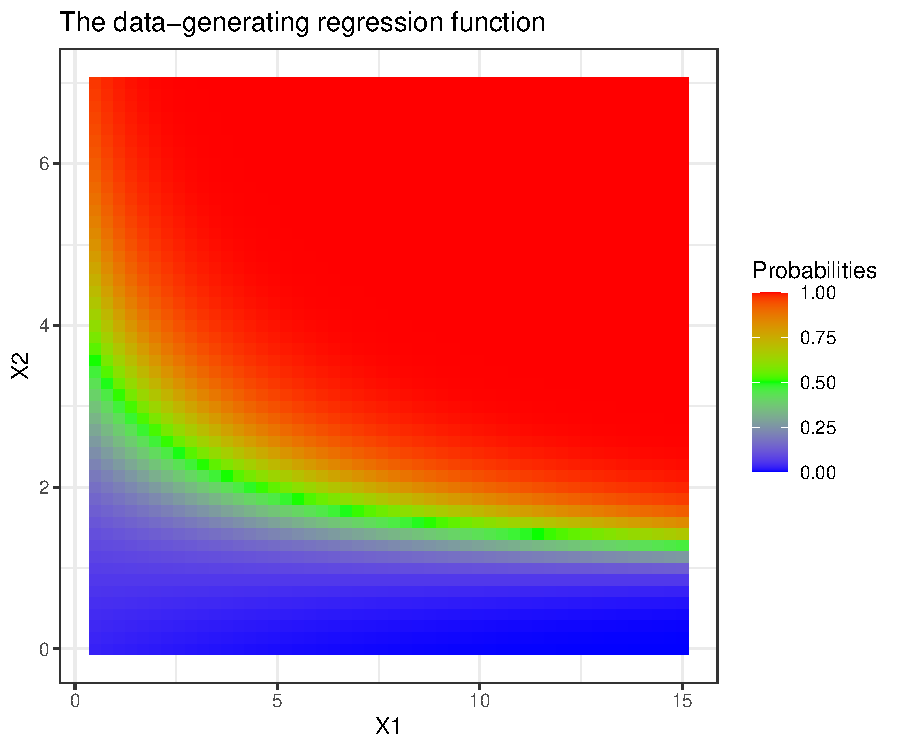
\includegraphics[width=0.8\textwidth]{figures/trueplot.pdf}
    \caption{The true regression plotted as a heat map. The two covariates $ X_1 $ and $ X_2 $ are mapped by the regression function $ \theta_0 $ to a probability as indicated by the colors.}
    \label{fig:trueplot}
\end{figure}
\end{frame}


\begin{frame}
    \frametitle{Simulations: Library of Algorithms} 
The regression is captured by using logistic regression with interaction terms. We use the following library of learning algorithms:
\begin{enumerate}
    \item Intercept only logistic regression: $E[Y \mid X_1, X_2] = \expit(\beta_0)$
    \item Logistic regression with main effects: $E[Y \mid X_1, X_2] = \expit(\beta_0 + \beta_1 X_1 + \beta_2 X_2)$
    \item XGBoost with hyperparameters: \texttt{max\_depth=3, eta=0.3,\\ n\_rounds=100, objective='binary:logistic', booster='dart', nthread=5}
\end{enumerate}
The intercept model is included as a \textbf{benchmark}, no learning algorithm should perform worse than the benchmark. 
\note[item]{The true regression is captured by logistic regression with interaction terms, and we will consider the following library as an example}

\note[item]{We have an intercept logistic regression which is included as a benchmark, the logistic regression with only main effects terms and no interaction, and XGBoost with hyperparameters }

\note[item]{The intercept model is included as a benchmark, so no learning algorithm should perform worse than the benchmark}
\end{frame}

\begin{frame}
    \frametitle{Simulations: Logistic Regression and XGBoost} 
    \begin{figure}
        \centering
        \centerline{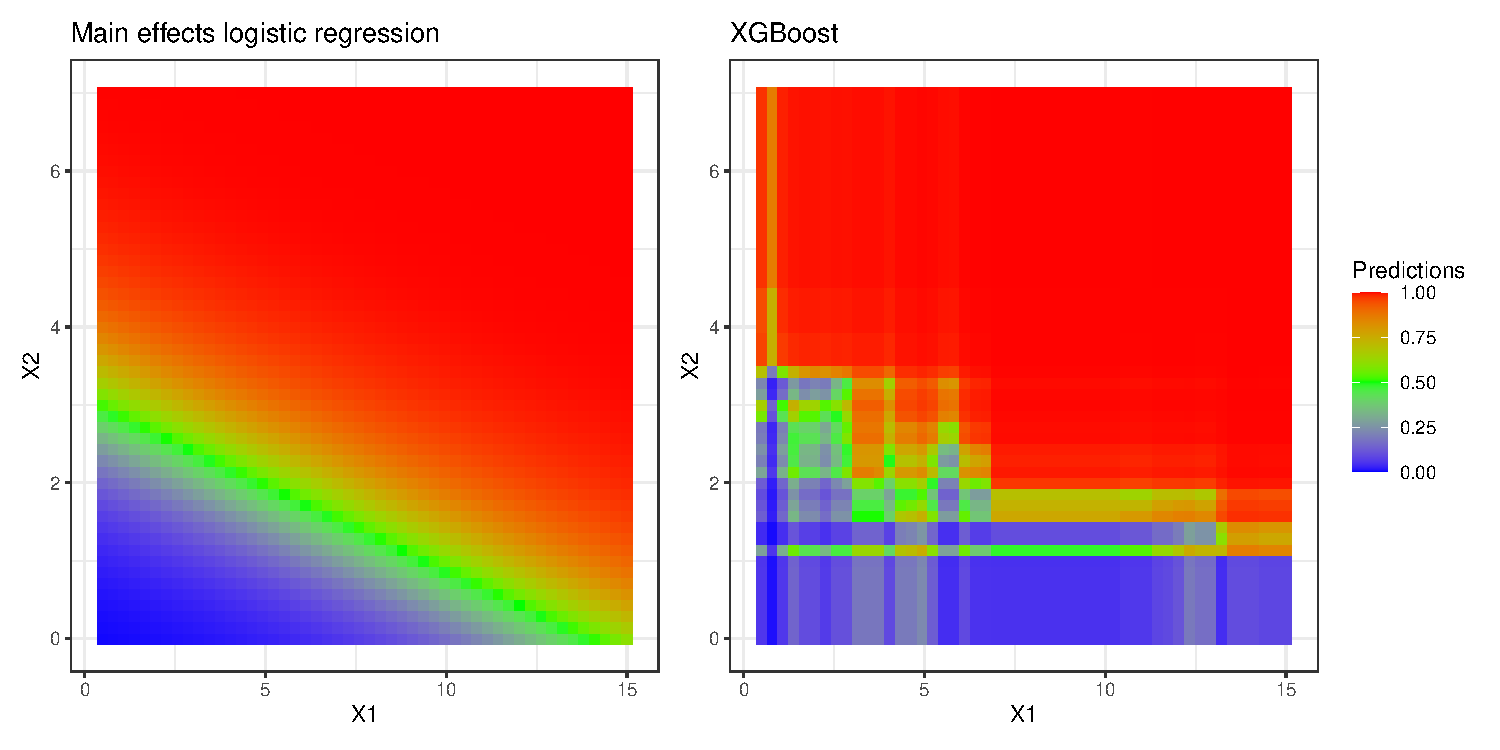
\includegraphics[width=1.1\textwidth]{figures/predictpar.pdf}}
        \caption{The predictions of the main effects logistic regression and XGBoost fitted on $ 1,000 $ observations.}
        \label{fig:predictpar}
    \end{figure}
    \note[item]{These plots are from the third slide from before, and we see that the main effects model is very biased and cannot model the interaction effect between two covariates}
    \note[item]{XGBoost predicts a patchy patterm, which becomes smoother as we fit with more samples, fitting on 10,000 observations yields the following plot}
\end{frame}

\begin{frame}
    \begin{figure}[H]
        \centering
        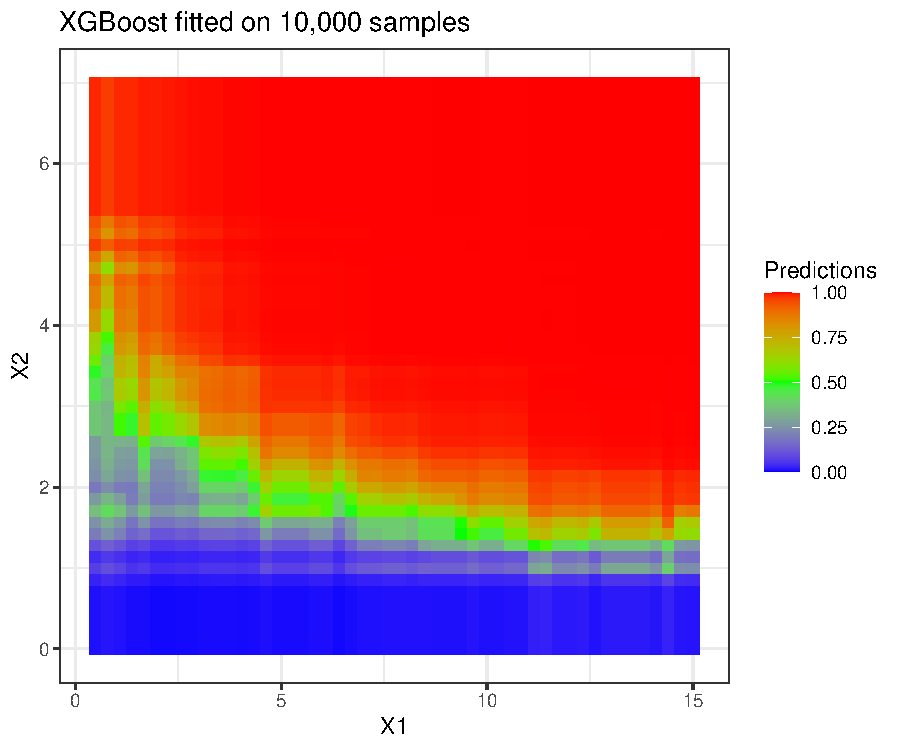
\includegraphics[width=0.8\textwidth]{figures/xgboost10k.pdf}
        \caption{XGBoost becoming better at approximating the regression as the sample size increases. Here the predictions of XGBoost are visualized for a training sample size of $ 10,000 $. }
        \label{fig:xgboost10k}
    \end{figure}
\end{frame}

\begin{frame}
    \begin{figure}[H]
        \centering
        \centerline{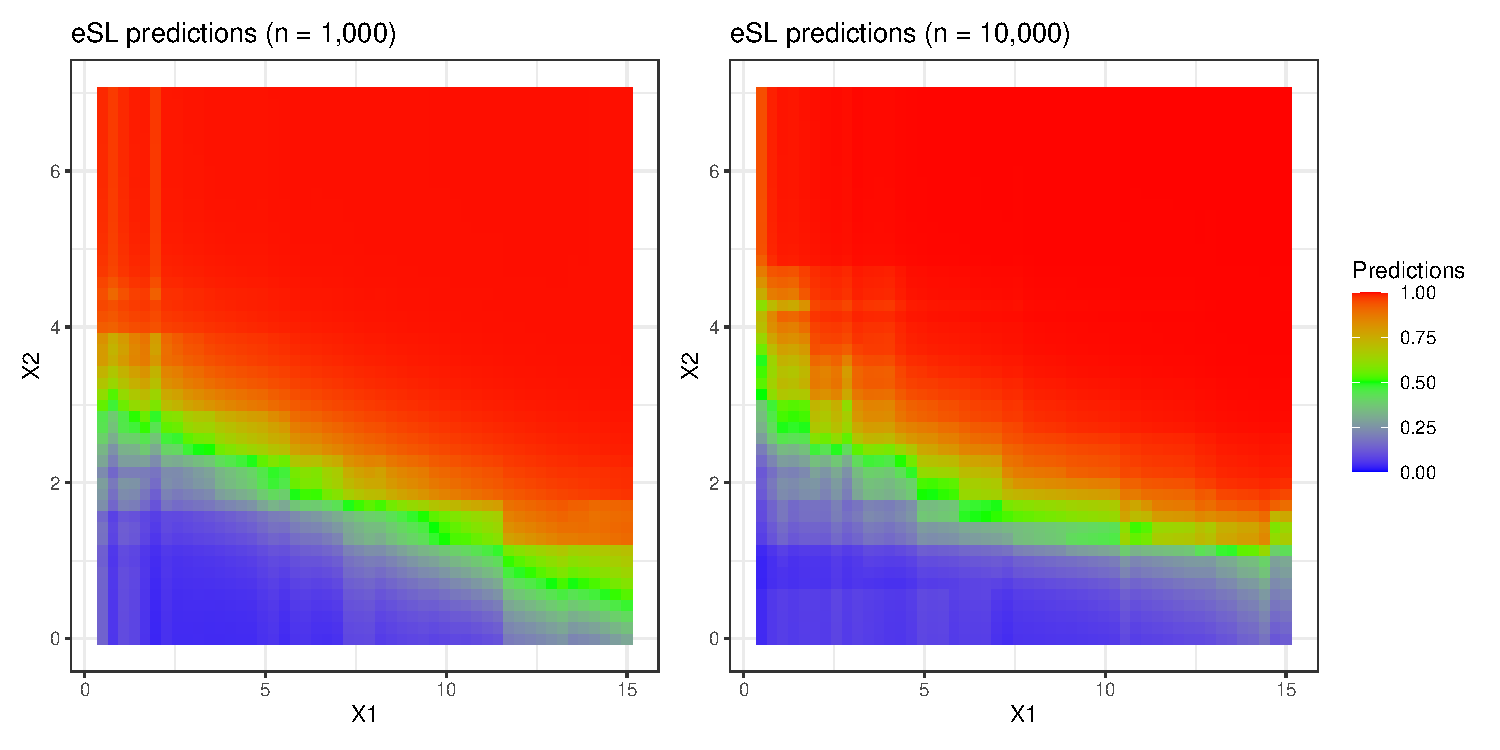
\includegraphics[width=1.1\textwidth]{figures/esl_preds_par.pdf}}
        \caption{The predictions by the ensemble super learner using the constrained regression meta learning algorithm fitted on $ 1,000 $ and $ 10,000 $ observations.}
        \label{fig:esl_preds_quad_prog}
    \end{figure}
    \note[item]{The ensemble super learner combines the learner predictions, and as we see in the following plots, it seems that it is indeed a blend of the smooth parametric logistic regression and the patchy pattern of xgboost}

    \note[item]{We see that there is some gradient where the predictions are around 0.5, intertwined with the patchiness characteristic of XGBoost}
\end{frame}


\subsection{Validation risk and variance}
\begin{frame}
    \frametitle{Simulations: Risk and Variance over Training Samples} 
    \begin{figure}[H]
        \centering
        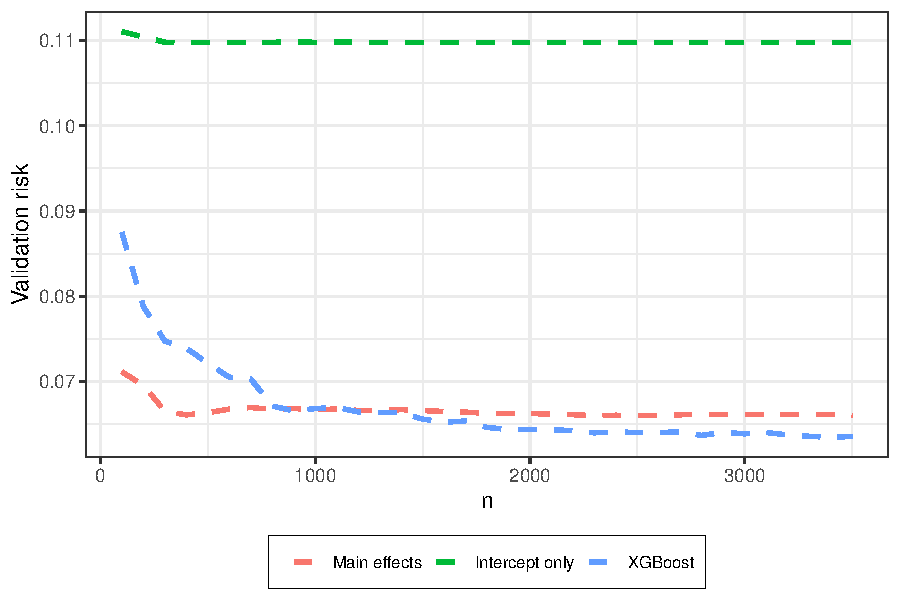
\includegraphics[width=0.87\textwidth]{figures/losses_candidates.pdf}
        \caption{The validation risk of the learning algorithms where training samples are $n = 100, 200, \dots , N = 3,500 $.}
        \label{fig:losses_candidates}
    \end{figure}
    \note[item]{Here we have plotted validation risks over the number of training samples, the validation risks are calculated by sampling 10000 observations from the true distribution, each algorithm is fitted on n observations and an empirical risk is calculated on the validation set}

    \note[item]{We see that the validation risk for XGBoost steadily decreases, whereas for the the logistic regression it appears quite stable}

    \note[item]{We also notice that XGBoost has a high validation risk for low samples, which is characteristic of machine learning methods that are very flexible, and can fit all sorts of distributions}

    \note[item]{It makes sense that since XGBoost has not been trained on as much data, then the validation risk is necessarily higher}

    \note[item]{XGboost eventually beats the main effects logistic regression when the number of training samples increase}
\end{frame}

\begin{frame}
    \begin{figure}[H]
        \centering
        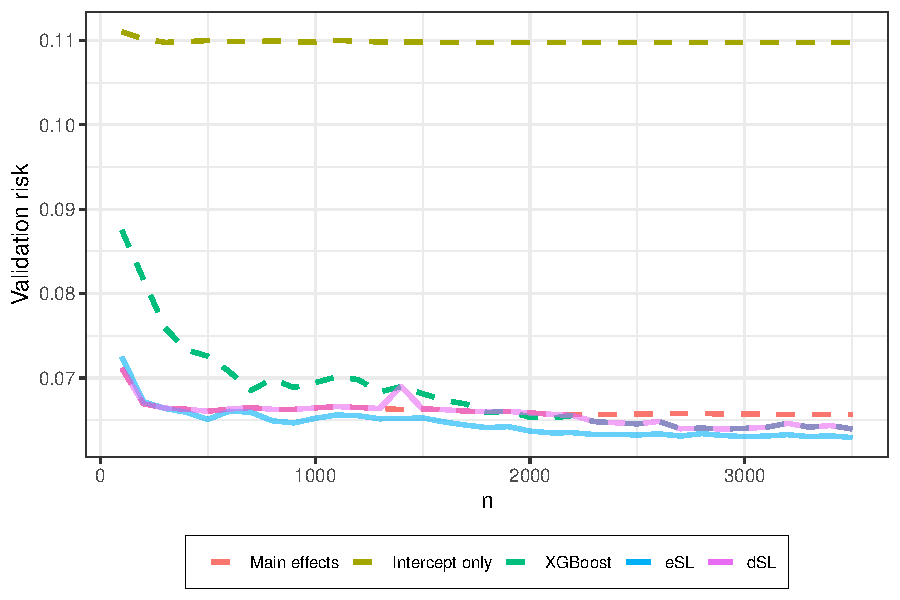
\includegraphics[width=0.87\textwidth]{figures/losses_candidates_sl.pdf}
        \caption{The validation risk of the super learners compared to the library of algorithms where the number of training samples are $n = 100, 200, \dots , N = 3,500 $.}
        \label{fig:losses_esl_s22}
    \end{figure}

    \note[item]{Here is a plot where the validation risks of the super learners are included}

    \note[item]{The pink line, representing the discrete super learner, has the same risk to the main effects model for small samples. However, as the sample size grows and the risk of XGBoost becomes smaller, the risk of the discrete super learner aligns with that of XGBoost.}

    \note[item]{This is in line with the fact that the discrete super learner selects a learner from the library, and hence the minimum risk that it can achieve must be the risk of one of the learners}

    \note[item]{The ensemble super learner in blue, is a combination of different learners achieves a risk that is strictly lower than all learners including the discrete super learner}
\end{frame}

\begin{frame}
\begin{figure}[H]
    \centering
    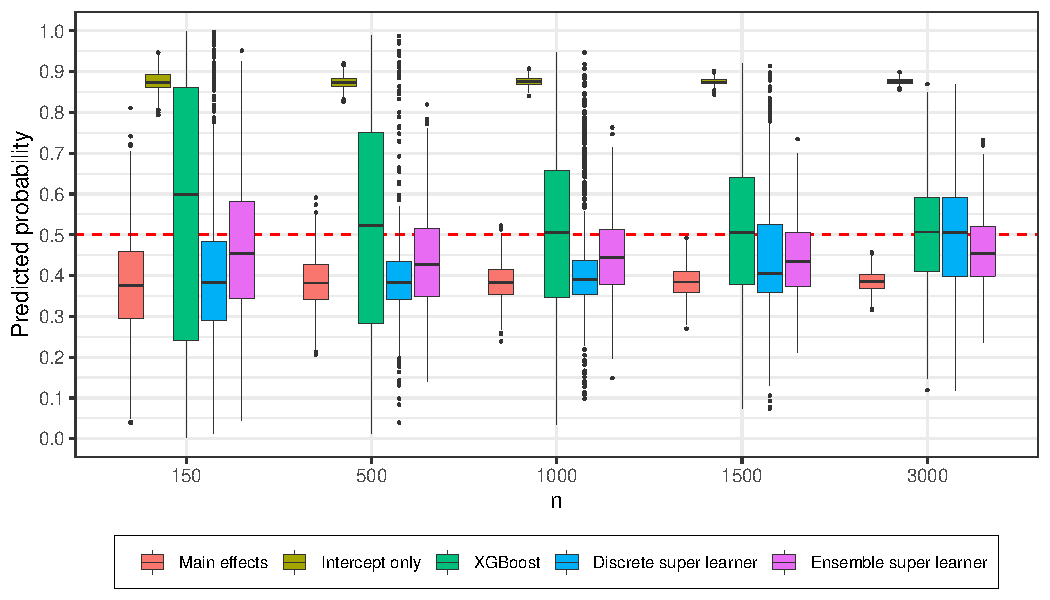
\includegraphics[width=\textwidth]{figures/learner_vars_w_esl_1000.pdf}
    \caption{The variances of the super learners compared to other algorithms. Each algorithm is fitted $ K = 1,000 $ times on $n$ samples and used to predict $ K $ times on a single observation.}
    \label{fig:learner_vars_w_esl_1000}
\end{figure}

    \note[item]{In this plot we have fitted each algorithm 1000 times on n samples as indicated on the horizontal axis, and each time they are fitted, they are used to predict on a single fixed observation whose true probability is 0.5 }

    \note[item]{We see that the variance of XGBoost is extremely high, ranging from 0.1 to 0.9 for a single observation}

    \note[item]{In comparison, the logistic regression models achieve a much lower variance, but are in turn heavily biased}

    \note[item]{which illustrates the bias-variance tradeoff between using data-adaptive machine learning methods and parametric methods such as logistic regression}

    \note[item]{An interesting observation here is that the ensemble super learner, which is a combination of the learners, is not as biased as the logistic regression, but has a higher variance, though less than XGBoost}
\end{frame}




\subsection{Locally weighted eSL}
\begin{frame}
    \frametitle{Locally Weighted Ensemble Super Learner} 
    \begin{figure}[H]
        \centering
        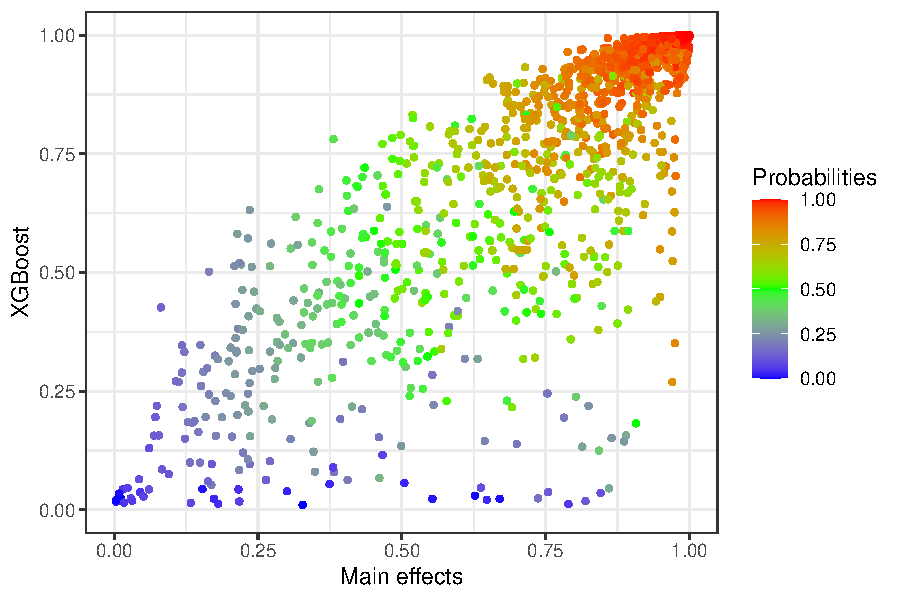
\includegraphics[width=0.8\textwidth]{figures/esl_preds_xgboost_vs_main.pdf}
        \caption{Predictions of XGBoost vs main effects model in level 1 covariates. The learners' prediction on a single observation represent a point in the unit square, the point is colored by the probability obtained from applying the true regression function on that observation.}
        \label{fig:esl_preds_xgboost_vs_main}
    \end{figure}

    \note[item]{i will now introduce the locally weighted ensemble super learner is my own extension }

    \note[item]{Here i have visualized the predictions of XGBoost vs Main effects, each point represents an observation, and is colored by their true probabilities, the axes indicate the predictions of the two learning algorithms}

    \note[item]{We see that XGBoost and the main effects model disagree significantly on some observations}

    \note[item]{For example as seen in the lower right corner, the main effects sometimes predicts the probability to be around 0.7 whereas XGBoost predicts to be around 0.1}

    \note[item]{One idea would be to weigh certain learners more than others in certain regions, for example we might weigh XGBoost a lot more in the lower right corner as it seems to be more accurate}
\end{frame}


\begin{frame}
    \frametitle{Clustering level 1 covariates using $ k $-means} 
    \begin{figure}[H]
        \centering
        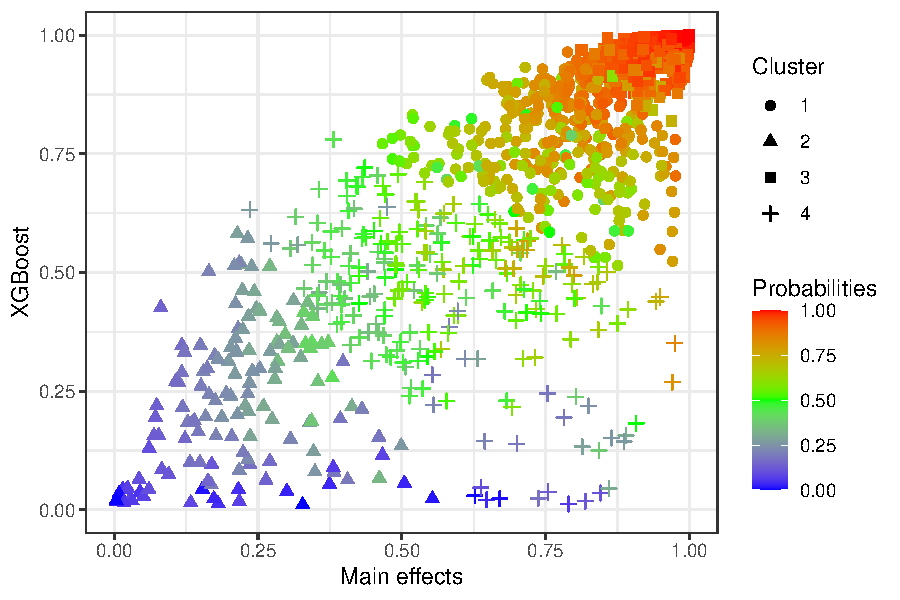
\includegraphics[width=0.8\textwidth]{figures/esl_preds_xgboost_vs_main_kmeans.pdf}
    \caption{The predictions are clustered into 4 groups using $ k $-means clustering.}
        \label{fig:esl_preds_xgboost_vs_main_kmeans}
    \end{figure}

    \note[item]{Here I have used k-means clustering to cluster the level-1 covariates into 4 groups, for each group, an ensemble super learner is used combines the predictions using weights specifically fitted for that group}
\end{frame}

\begin{frame}
    \begin{figure}[H]
        \centering
        \centerline{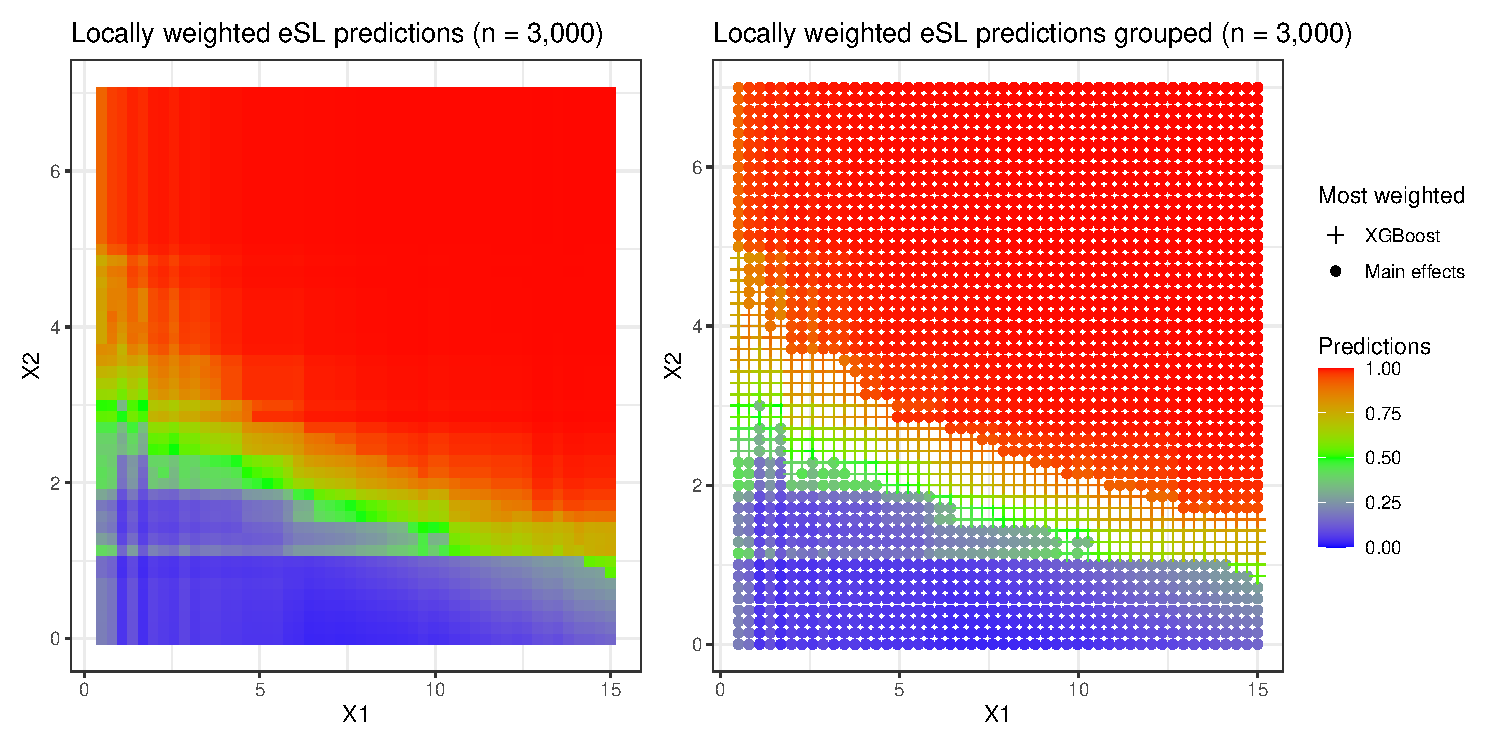
\includegraphics[width=1.1\textwidth]{figures/esl_preds_lw_stratified_tiled5.pdf}}
        \caption{Predictions of locally weighted ensemble super learner, where the predictions of XGBoost have highest weight when $ p \approx 0.5 $}
        \label{fig:esl_preds_lw_stratified_tiled5}
    \end{figure}
    \note[item]{One can then stratify the predicted probabilities according to the learner that was weighed the most }

    \note[item]{Here XGBoost has the highest weight when the predicted probability is around 0.5 which is quite interesting to see}

    \note[item]{It seems also that there is a clearer gradient when going from 0.5 to 0.7}
\end{frame}

\section{Concluding Remarks}
\begin{frame}
    \frametitle{Concluding Remarks} 
    \begin{enumerate}
        \item<1-> Oracle property also holds for the ensemble super learner
            \note[item]<1>{Similar oracle property holds for the ensemble super learner which is a minor extension to the oracle result of the discrete super learner }
        \item<2-> How can we make machine learning methods more stable? 
            \note[item]<2>{As we have seen with the machine learning method XGBoost, it has an extremely high variance unless one has a lot of observations. The high variance results in undesirable irregular patchy predictions which does not model the data-generating distribution}

            \note[item]<2>{The locally weighted ensemble super learner was an attempt at smoothening the irregular predictions of XGBoost by combining it with a parametric method such as logistic regression}
            \note[item]<2>{My hope was that by weighing the parametric regression more in certain regions, one can selectively ignore the noisy predictions from XGBoost, but still retain its more accurate predictions that the parametric regression could not capture}

        \item<3-> The ensemble super learner seeks to balance the bias-variance tradeoff 
            $$R(\btheta, P) = E(\btheta(X) - m(X))^2 + E(m(X) - Y)^2$$
            $$E(\btheta(X) - m(X))^2 = \operatorname{Var}(\btheta(X)) + \operatorname{Bias}(\btheta(X))^2 $$ where $ m $ is the true regression
            \note[item]<3>{Finally, if we consider the ensemble super learner with the quadratic risk function, then one can argue that it attempts to select the most optimal weighting scheme that balances the bias-variance tradeoff}

            \note[item]<3>{It is well-known that the quadratic risk has the following decomposition}

            \note[item]<3>{So by minimizing the quadratic risk over theta, we are minimizing the first the term which can decomposed into the variance of theta plus its squared bias}
    \end{enumerate}
\end{frame}
 

\end{document}
